\documentclass{ximera}  


%\usepackage{todonotes}
%\usepackage{mathtools} %% Required for wide table Curl and Greens
%\usepackage{cuted} %% Required for wide table Curl and Greens
\newcommand{\todo}{}

\usepackage{esint} % for \oiint
\ifxake%%https://math.meta.stackexchange.com/questions/9973/how-do-you-render-a-closed-surface-double-integral
\renewcommand{\oiint}{{\large\bigcirc}\kern-1.56em\iint}
\fi


\graphicspath{
  {./}
  {jpg}
  {ximeraTutorial/}
  {basicPhilosophy/}
  {functionsOfSeveralVariables/}
  {normalVectors/}
  {lagrangeMultipliers/}
  {vectorFields/}
  {greensTheorem/}
  {shapeOfThingsToCome/}
  {dotProducts/}
  {partialDerivativesAndTheGradientVector/}
  {../productAndQuotientRules/exercises/}
  {../motionAndPathsInSpace/exercises/}
  {../normalVectors/exercisesParametricPlots/}
  {../continuityOfFunctionsOfSeveralVariables/exercises/}
  {../partialDerivativesAndTheGradientVector/exercises/}
  {../directionalDerivativeAndChainRule/exercises/}
  {../commonCoordinates/exercisesCylindricalCoordinates/}
  {../commonCoordinates/exercisesSphericalCoordinates/}
  {../greensTheorem/exercisesCurlAndLineIntegrals/}
  {../greensTheorem/exercisesDivergenceAndLineIntegrals/}
  {../shapeOfThingsToCome/exercisesDivergenceTheorem/}
  {../greensTheorem/}
  {../shapeOfThingsToCome/}
  {../separableDifferentialEquations/exercises/}
  {vectorFields/}
}

\newcommand{\mooculus}{\textsf{\textbf{MOOC}\textnormal{\textsf{ULUS}}}}

\usepackage{tkz-euclide}\usepackage{tikz}
\usepackage{tikz-cd}
\usetikzlibrary{arrows}
\tikzset{>=stealth,commutative diagrams/.cd,
  arrow style=tikz,diagrams={>=stealth}} %% cool arrow head
\tikzset{shorten <>/.style={ shorten >=#1, shorten <=#1 } } %% allows shorter vectors

\usetikzlibrary{backgrounds} %% for boxes around graphs
\usetikzlibrary{shapes,positioning}  %% Clouds and stars
\usetikzlibrary{matrix} %% for matrix
\usepgfplotslibrary{polar} %% for polar plots
\usepgfplotslibrary{fillbetween} %% to shade area between curves in TikZ
\usetkzobj{all}
\usepackage[makeroom]{cancel} %% for strike outs
%\usepackage{mathtools} %% for pretty underbrace % Breaks Ximera
%\usepackage{multicol}
\usepackage{pgffor} %% required for integral for loops



%% http://tex.stackexchange.com/questions/66490/drawing-a-tikz-arc-specifying-the-center
%% Draws beach ball
\tikzset{pics/carc/.style args={#1:#2:#3}{code={\draw[pic actions] (#1:#3) arc(#1:#2:#3);}}}



\usepackage{array}
\setlength{\extrarowheight}{+.1cm}
\newdimen\digitwidth
\settowidth\digitwidth{9}
\def\divrule#1#2{
\noalign{\moveright#1\digitwidth
\vbox{\hrule width#2\digitwidth}}}





\newcommand{\RR}{\mathbb R}
\newcommand{\R}{\mathbb R}
\newcommand{\N}{\mathbb N}
\newcommand{\Z}{\mathbb Z}

\newcommand{\sagemath}{\textsf{SageMath}}


%\renewcommand{\d}{\,d\!}
\renewcommand{\d}{\mathop{}\!d}
\newcommand{\dd}[2][]{\frac{\d #1}{\d #2}}
\newcommand{\pp}[2][]{\frac{\partial #1}{\partial #2}}
\renewcommand{\l}{\ell}
\newcommand{\ddx}{\frac{d}{\d x}}

\newcommand{\zeroOverZero}{\ensuremath{\boldsymbol{\tfrac{0}{0}}}}
\newcommand{\inftyOverInfty}{\ensuremath{\boldsymbol{\tfrac{\infty}{\infty}}}}
\newcommand{\zeroOverInfty}{\ensuremath{\boldsymbol{\tfrac{0}{\infty}}}}
\newcommand{\zeroTimesInfty}{\ensuremath{\small\boldsymbol{0\cdot \infty}}}
\newcommand{\inftyMinusInfty}{\ensuremath{\small\boldsymbol{\infty - \infty}}}
\newcommand{\oneToInfty}{\ensuremath{\boldsymbol{1^\infty}}}
\newcommand{\zeroToZero}{\ensuremath{\boldsymbol{0^0}}}
\newcommand{\inftyToZero}{\ensuremath{\boldsymbol{\infty^0}}}



\newcommand{\numOverZero}{\ensuremath{\boldsymbol{\tfrac{\#}{0}}}}
\newcommand{\dfn}{\textbf}
%\newcommand{\unit}{\,\mathrm}
\newcommand{\unit}{\mathop{}\!\mathrm}
\newcommand{\eval}[1]{\bigg[ #1 \bigg]}
\newcommand{\seq}[1]{\left( #1 \right)}
\renewcommand{\epsilon}{\varepsilon}
\renewcommand{\phi}{\varphi}


\renewcommand{\iff}{\Leftrightarrow}

\DeclareMathOperator{\arccot}{arccot}
\DeclareMathOperator{\arcsec}{arcsec}
\DeclareMathOperator{\arccsc}{arccsc}
\DeclareMathOperator{\si}{Si}
\DeclareMathOperator{\scal}{scal}
\DeclareMathOperator{\sign}{sign}


%% \newcommand{\tightoverset}[2]{% for arrow vec
%%   \mathop{#2}\limits^{\vbox to -.5ex{\kern-0.75ex\hbox{$#1$}\vss}}}
\newcommand{\arrowvec}[1]{{\overset{\rightharpoonup}{#1}}}
%\renewcommand{\vec}[1]{\arrowvec{\mathbf{#1}}}
\renewcommand{\vec}[1]{{\overset{\boldsymbol{\rightharpoonup}}{\mathbf{#1}}}\hspace{0in}}

\newcommand{\point}[1]{\left(#1\right)} %this allows \vector{ to be changed to \vector{ with a quick find and replace
\newcommand{\pt}[1]{\mathbf{#1}} %this allows \vec{ to be changed to \vec{ with a quick find and replace
\newcommand{\Lim}[2]{\lim_{\point{#1} \to \point{#2}}} %Bart, I changed this to point since I want to use it.  It runs through both of the exercise and exerciseE files in limits section, which is why it was in each document to start with.

\DeclareMathOperator{\proj}{\mathbf{proj}}
\newcommand{\veci}{{\boldsymbol{\hat{\imath}}}}
\newcommand{\vecj}{{\boldsymbol{\hat{\jmath}}}}
\newcommand{\veck}{{\boldsymbol{\hat{k}}}}
\newcommand{\vecl}{\vec{\boldsymbol{\l}}}
\newcommand{\uvec}[1]{\mathbf{\hat{#1}}}
\newcommand{\utan}{\mathbf{\hat{t}}}
\newcommand{\unormal}{\mathbf{\hat{n}}}
\newcommand{\ubinormal}{\mathbf{\hat{b}}}

\newcommand{\dotp}{\bullet}
\newcommand{\cross}{\boldsymbol\times}
\newcommand{\grad}{\boldsymbol\nabla}
\newcommand{\divergence}{\grad\dotp}
\newcommand{\curl}{\grad\cross}
%\DeclareMathOperator{\divergence}{divergence}
%\DeclareMathOperator{\curl}[1]{\grad\cross #1}
\newcommand{\lto}{\mathop{\longrightarrow\,}\limits}

\renewcommand{\bar}{\overline}

\colorlet{textColor}{black}
\colorlet{background}{white}
\colorlet{penColor}{blue!50!black} % Color of a curve in a plot
\colorlet{penColor2}{red!50!black}% Color of a curve in a plot
\colorlet{penColor3}{red!50!blue} % Color of a curve in a plot
\colorlet{penColor4}{green!50!black} % Color of a curve in a plot
\colorlet{penColor5}{orange!80!black} % Color of a curve in a plot
\colorlet{penColor6}{yellow!70!black} % Color of a curve in a plot
\colorlet{fill1}{penColor!20} % Color of fill in a plot
\colorlet{fill2}{penColor2!20} % Color of fill in a plot
\colorlet{fillp}{fill1} % Color of positive area
\colorlet{filln}{penColor2!20} % Color of negative area
\colorlet{fill3}{penColor3!20} % Fill
\colorlet{fill4}{penColor4!20} % Fill
\colorlet{fill5}{penColor5!20} % Fill
\colorlet{gridColor}{gray!50} % Color of grid in a plot

\newcommand{\surfaceColor}{violet}
\newcommand{\surfaceColorTwo}{redyellow}
\newcommand{\sliceColor}{greenyellow}




\pgfmathdeclarefunction{gauss}{2}{% gives gaussian
  \pgfmathparse{1/(#2*sqrt(2*pi))*exp(-((x-#1)^2)/(2*#2^2))}%
}


%%%%%%%%%%%%%
%% Vectors
%%%%%%%%%%%%%

%% Simple horiz vectors
\renewcommand{\vector}[1]{\left\langle #1\right\rangle}


%% %% Complex Horiz Vectors with angle brackets
%% \makeatletter
%% \renewcommand{\vector}[2][ , ]{\left\langle%
%%   \def\nextitem{\def\nextitem{#1}}%
%%   \@for \el:=#2\do{\nextitem\el}\right\rangle%
%% }
%% \makeatother

%% %% Vertical Vectors
%% \def\vector#1{\begin{bmatrix}\vecListA#1,,\end{bmatrix}}
%% \def\vecListA#1,{\if,#1,\else #1\cr \expandafter \vecListA \fi}

%%%%%%%%%%%%%
%% End of vectors
%%%%%%%%%%%%%

%\newcommand{\fullwidth}{}
%\newcommand{\normalwidth}{}



%% makes a snazzy t-chart for evaluating functions
%\newenvironment{tchart}{\rowcolors{2}{}{background!90!textColor}\array}{\endarray}

%%This is to help with formatting on future title pages.
\newenvironment{sectionOutcomes}{}{}



%% Flowchart stuff
%\tikzstyle{startstop} = [rectangle, rounded corners, minimum width=3cm, minimum height=1cm,text centered, draw=black]
%\tikzstyle{question} = [rectangle, minimum width=3cm, minimum height=1cm, text centered, draw=black]
%\tikzstyle{decision} = [trapezium, trapezium left angle=70, trapezium right angle=110, minimum width=3cm, minimum height=1cm, text centered, draw=black]
%\tikzstyle{question} = [rectangle, rounded corners, minimum width=3cm, minimum height=1cm,text centered, draw=black]
%\tikzstyle{process} = [rectangle, minimum width=3cm, minimum height=1cm, text centered, draw=black]
%\tikzstyle{decision} = [trapezium, trapezium left angle=70, trapezium right angle=110, minimum width=3cm, minimum height=1cm, text centered, draw=black]




 
\title{Traveling and Standing Waves} 
\author{Milica Markovic} 
\outcome{}
\begin{document}  
\begin{abstract}  

\end{abstract}  
\maketitle    





\section{Standing Waves}


In the previous section, we introduced the voltage reflection coefficient that relates the forward to reflected voltage phasor.

\begin{eqnarray}
\tilde{V}(z)= \tilde{V}_0^+ (e^{-j \beta z} + \Gamma_L  e^{j \beta z }  ) \label{eq:vtlfin} \\
I(z)=   \frac{\tilde{V}_0^+}{Z_0}  (e^{-j \beta z} - \Gamma_L  e^{j \beta z}  ) \label{eq:itlfin}
\end{eqnarray}


 Let us look at the physical meaning of these variables.

\begin{enumerate}
\item $\Gamma_L$ is the voltage reflection coefficient at the load (z=0), 
\item $z$ is the axis in
the direction of wave propagation, 
\item $\beta$ is the phase
constant,
\item $Z_0$ is the impedance of the transmission line. 
\item $\tilde{V}_0^+$ is the phasor of the forward-going wave at the load,
\item $\Gamma _L \tilde{V}_0^+$ is the phasor of the reflected going wave at the load,
\item $\tilde{V}_0^+ e^{-j \beta z} $ is a forward voltage anywhere on the line, 
 \item $ \Gamma _L \tilde{V}_0^+ e^{j \beta z} $ is a reflected voltage anywhere on the line, 
\item $\tilde{V}(z)$ is the total voltage phasor on the line, the sum of forward and reflected voltage.
\item $\tilde{I}_0^+$ is the phasor of the forward-going current  at the load,
\item $-\Gamma _L \frac{\tilde{V}_0^+}{Z_0}$ is the phasor of the reflected current at the load,
\item $\tilde{I}_0^+ e^{-j \beta z} $ is the phasor of a forward current  anywhere on the line, 
 \item $-\Gamma _L \frac{\tilde{V}_0^+}{Z_0} e^{j \beta z} $ is the phasor of a reflected current anywhere on the line, 
\item $\tilde{I}(z)$ is the phasor of the total current on the line, the sum of forward and reflected voltage.
\end{enumerate}
 


The magnitude of a complex number can be found as $|z|=\sqrt{z
z^*}$.Therefore  the magnitude of the voltage anywhere on the line is $|\tilde{V}(z)|=\sqrt{\tilde{V}(z)
\tilde{V}(z)^*}$. We can simplify this equation as shown in Figure \ref{eq:SWsw1}.

\begin{eqnarray}
|\tilde{V}(z)|=\sqrt{\tilde{V}(z) \tilde{V}(z)^*} \nonumber  \\
|\tilde{V}(z)|=\sqrt{   (\tilde{V}_0^+)^2 (e^{-j \beta z} - |\Gamma_L|  e^{j \beta z +
 \Theta_r}  )  
   \tilde{V}_0^+ (e^{j \beta z} - |\Gamma_L|  e^{-(j \beta z + \angle \Gamma_L)}     )} \nonumber
\\
|\tilde{V}(z)|= \tilde{V}_0^+ \sqrt{(e^{-j \beta z} - |\Gamma_L|  e^{j \beta z +
|\angle \Gamma_L}  )  
  (e^{j \beta z} - |\Gamma_L|  e^{-(j \beta z + \angle \Gamma_L)}     )}
\nonumber \\
|\tilde{V}(z)|= \tilde{V}_0^+ \sqrt{1+  |\Gamma_L|  e^{-(2j \beta z +
|\angle \Gamma_L)}    + |\Gamma_L|  e^{j 2 \beta z + \angle \Gamma_L} +|\Gamma_L|^2     )}
\nonumber \\
|\tilde{V}(z)|= \tilde{V}_0^+ \sqrt{1+ |\Gamma_L|^2 + |\Gamma_L| ( e^{-(2j \beta z +
 \angle \Gamma_L)} \angle \Gamma_L  +  e^{(j 2 \beta z + \angle \Gamma_L)}     )}
 \nonumber \\
|\tilde{V}(z)|= \tilde{V}_0^+  \sqrt{1+ |\Gamma_L|^2 + 2 |\Gamma_L| \cos(2 \beta z +\angle \Gamma_L)} \label{eq:SWsw1} 
\end{eqnarray}

The Equation \ref{eq:SWsw1} is written in terms of $z$. We set up the load at $z=0$, and the generator at $z=-l$. The positions of the maximums and minimum total voltage on the line will be at some position at the negative part of z-axis $z_{max}=-l_{max}$, and the minimums will be at $z_{max}=-l_{min}$.

The magnitude of the total voltage on the transmission line is given
by Eq.\ref{eq:SWsw1}. We will now visualize how the magnitude of the voltage looks on the transmission line.


\begin{example}

Find the magnitude of the total voltage anywhere on the transmission line if $\Gamma_L=0$.

\begin{explanation}
 Let us start from a simple case when the voltage reflection coefficient on the
transmission line is $\Gamma_L=0$ and draw the magnitude of the total
voltage as a function of z. Equation \ref{eq:SWsw1} shows the magnitude of the total voltage anywhere on the line is equal to the magnitude of the voltage at the load $|\tilde{V}(z)|= |\tilde{V}_0^+|$.  The magnitude of the voltage is constant everywhere on the transmission line, and so the line
is called "flat," and it represents a single, forward traveling wave from the generator to the load. The magnitude is the green line in Figure \ref{fig:SWflatline}. To see the movie
of this transmission line, go to the class web page under Instructional Videos. Forward voltage is shown in red, reflected voltage in pink,
and the magnitude of the voltage is green.




\begin{figure}[htbp]
\begin{center}
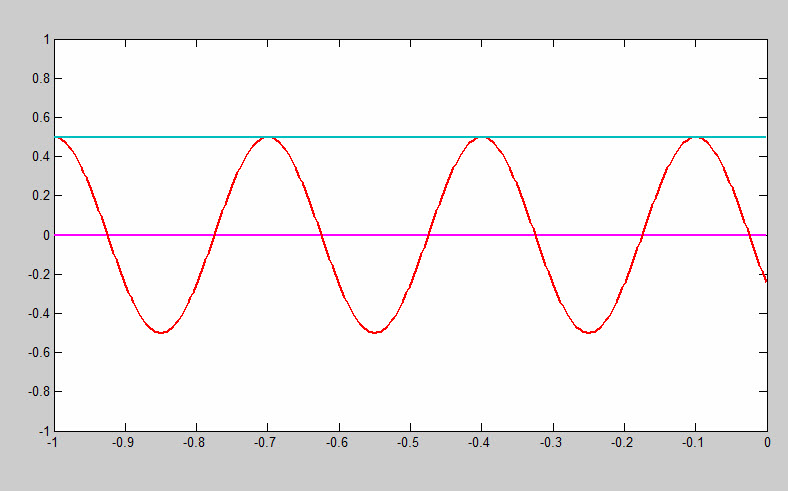
\includegraphics[scale=0.3]{../jpg/flatline.jpg}
%\strut\psfig{figure=smithchartreflection.ps,width=3cm} \\
\end{center}
\caption{Flat line.}
\label{fig:SWflatline}
\end{figure}
\end{explanation}

\end{example}


\begin{example}

Find the magnitude of the total voltage anywhere on the transmission line if $\Gamma_L=0.5 e^{j0}$.

\begin{explanation}
\item Let's look at another case,  $\Gamma_L=0.5$ and $\angle \Gamma_L=0$. Equation \ref{eq:SWswc1}  represents the magnitude of the voltage on the transmission line, and Figure \ref{fig:SWreflcoeffvid} shows in green how this function looks on a transmission line. This case is shown in Figure \ref{fig:SWreflcoeffvid}. 

\begin{eqnarray}
|\tilde{V}(z)|=\tilde{V}_0^+ \sqrt{\frac{5}{4}+ cos{2 \beta z} }\label{eq:SWswc1}
\end{eqnarray}

\begin{figure}[htbp]
\begin{center}
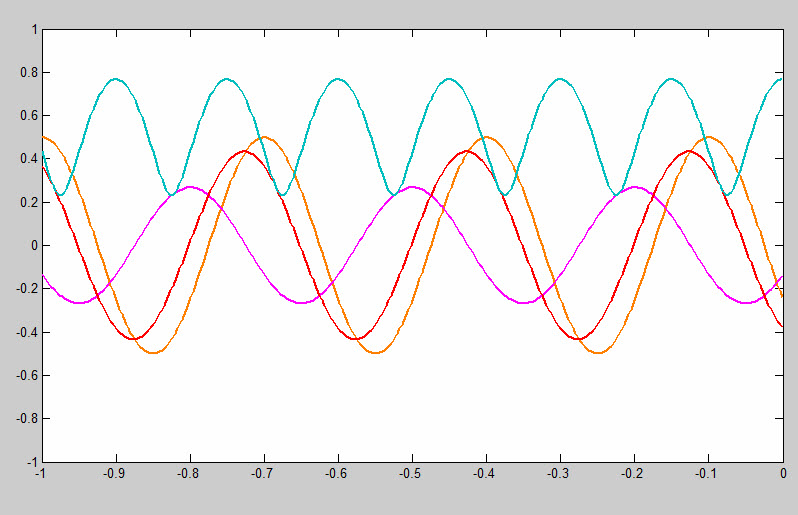
\includegraphics[scale=0.3]{specialcase.jpg}
%\strut\psfig{figure=smithchartreflection.ps,width=3cm} \\
\end{center}
\caption{Voltage on a transmission line with reflection coefficient magnitude 0.5, and zero phase.}
\label{fig:SWreflcoeffvid}
\end{figure}



The function in Equation \ref{eq:SWswc1} is at its maximum 
when $cos(2 \beta z+\angle \Gamma_L)=1$ or $z=\frac{k}{2} \lambda$, and the function
value is $\tilde{V}(z)=1.5\tilde{V}_0^+  $. It is at its
minimum when  $cos(2 \beta z+ \angle \Gamma_L)=-1$ or $z=\frac{2 k +1}{4} \lambda$
and the function value is $\tilde{V}(z)=0.5 \tilde{V}_0^+$

The function that we see looks
like a cosine with an average value of $ \tilde{V}_0^+ $, but {\bf it is not a cosine}.
The minimums of the function are sharper than the maximums. 



\end{explanation}
\end{example}


\begin{example}

Find the magnitude of the total voltage anywhere on the transmission line if $\Gamma_L=1$.

\begin{explanation}
Another case we will look at is when
the reflection coefficient is at its maximum of $\Gamma_L =1$. The
function is shown if Figure \ref{fig:SWStanding}. In this case, we have a pure standing wave on a transmission line.


\begin{figure}[htbp]
\begin{center}
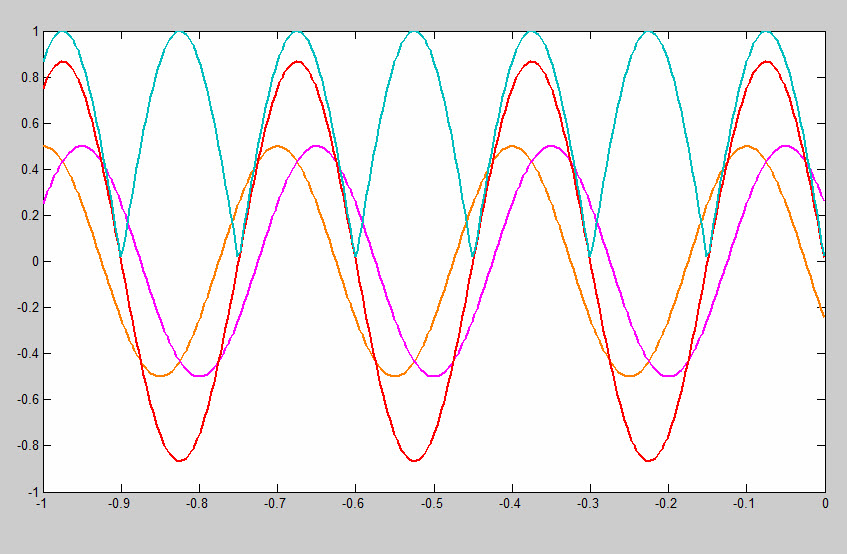
\includegraphics[scale=0.3]{../jpg/shortedline.jpg}
%\strut\psfig{figure=smithchartreflection.ps,width=3cm} \\
\end{center}
\caption{Shorted Transmission Line.}
\label{fig:SWStanding}
\end{figure}

\end{explanation}
\end{example}


\begin{example}

Find the magnitude of the total voltage anywhere on the transmission line for any $\Gamma_L$, and the position of voltage maximums on the line.
\begin{explanation}
 

The magnitude of the total voltage on the line is given in Equation\ref{eq:SWsw1}.  In general the voltage maximums will occur when the cosine function  is at its maximum
$cos(2 \beta z+\angle \Gamma_L)=1$. In this case, the maximum value of the magnitude of total voltage on the line is shown in Equation \ref{eq:SWMaxValue}.

\begin{eqnarray}
|\tilde{V}(z)_{max}|=|\tilde{V}_0^+|\sqrt{1+|\Gamma_L|^2+2 |\Gamma_L|} \nonumber  \\
|\tilde{V}(z)_{max}| =|\tilde{V}_0^+|\sqrt{(1+|\Gamma_L|)^2}  \nonumber \\
|\tilde{V}(z)_{max}| =|\tilde{V}_0^+|(1+|\Gamma_L|) \label{eq:SWMaxValue} 
\end{eqnarray}


The Equation \ref{eq:SWmaximums}  shows position of voltage maximums $z_{max}$ on the line. 
\begin{eqnarray}
cos(-2 \beta l_{max}+ \angle \Gamma_L)=1 \nonumber \\
cos(2 \beta l_{max}- \angle \Gamma_L)=1 \nonumber \\
2 \beta z_{max} - \angle \Gamma_L = 2 n \pi \nonumber \\
z_{max} =\frac{ 2 n \pi +\angle \Gamma_L }{ 2 \beta} \nonumber \\
z_{max}= \lambda \frac{ 2 n \pi +\angle \Gamma_L  }{ 4 \pi} \label{eq:SWmaximums}
\end{eqnarray}

In general the voltage minimums will occur when
$cos(2 \beta z)=-1$.
 

\begin{eqnarray}
|\tilde{V}(z)_{min}|=|\tilde{V}_0^+|\sqrt{1+|\Gamma_L|^2-2 |\Gamma_L|} \nonumber  \\
|\tilde{V}(z)_{min}| =|\tilde{V}_0^+|\sqrt{(1-|\Gamma_L|)^2}  \nonumber \\
|\tilde{V}(z)_{min}| =|\tilde{V}_0^+| (1-|\Gamma_L|) 
\end{eqnarray}

The Equation \ref{eq:SWminimums}  shows the position of voltage minimums on the line. 


\begin{eqnarray}
cos(2 \beta z_{max}-\angle \Gamma_L)=-1 \nonumber \\
2 \beta z_{max} + \angle \Gamma_L = (2 n+1) \pi \nonumber \\
z_{max} =\frac{ (2 n+1) \pi +\angle \Gamma_L }{ 2 \beta} \nonumber \\
z_{max}=\lambda \frac{ (2 n+1) \pi +\angle \Gamma_L  }{ 4 \pi} \label{eq:SWminimums}
\end{eqnarray}




\end{explanation}
\end{example}



\section{Voltage Standing Wave Ratio (VSWR) - pron: "vee-s-uh-ar"}





The ratio of voltage minimum on the line over the voltage maximum is
called the Voltage Standing Wave Ratio (VSWR) or just Standing Wave
Ratio (SWR).

\begin{eqnarray}
SWR=\frac{\tilde{V}(z)_{max}}{ \tilde{V}(z)_{min}} \nonumber \\
SWR=\frac{1+|\Gamma_L|}{1-|\Gamma_L|}
\end{eqnarray}


























\end{document} 
